\documentclass[a4paper, 10pt]{article}
\usepackage[utf8]{inputenc}
\usepackage[T1]{fontenc}
\usepackage{ngerman, lmodern}
%\usepackage[left=3cm, right=3cm]{geometry}

\newcommand{\mytitle}{Untersuchung und Kontrolle von chaotischem Verhalten am Doppelpendel}
\newcommand{\myauthor}{Jann Horn und Hannes Riechert}

\usepackage{graphicx, wrapfig, subfigure, color, amsmath, amsthm}
\usepackage{fancyhdr}
  \lhead{\myauthor}
  \chead{}
  \rhead{\nouppercase\leftmark}
  \lfoot{}
  \cfoot{\thepage}
  \rfoot{}

\usepackage[numbers]{natbib}
\usepackage{setspace}
  \onehalfspacing % Zeilenabstand
% \usepackage[numbers]{natbib} % bibliography

\newcommand{\TODO}{\textcolor{red}{ \textbf TODO }}
\newcommand{\mathematik}{\begin{equation*}\begin{aligned}}
\newcommand{\mathematikstop}{\end{aligned}\end{equation*}}
\renewcommand{\phi}{\varphi} % make "stroked" phi look "loopy"
\renewcommand{\rho}{\varrho}
\newcommand{\half}{\frac{1}{2}} % 1/2
\newcommand{\phid}{\dot{\phi}}  % phi with one dot
\newcommand{\intend}{\,\mathrm{d}} % end of integral
\newcommand{\EQU}{\qquad\bigg|\,} % separator for explanations for equivalent rearrangements

\clubpenalty = 10000
\widowpenalty = 10000
\displaywidowpenalty = 10000

\title{\mytitle}
\author{\myauthor}
%\date{ }

\begin{document}
\maketitle
\begin{abstract}
In unserem Projekt beschäftigen wir uns mit dem Verhalten von chaotischen Doppelpendeln. Wir wollen aus der aktuellen Bewegung eines Doppelpendels den weiteren Bewegungsablauf in einem kurzen Zeitintervall extrapolieren und dann versuchen, diese Bewegung zu beeinflussen.

Hierzu wollen wir zunächst ein Doppelpendel konstruieren, bei dem Daten über den aktuellen Bewegungszustand erfasst werden können. Diese Daten sollen in Echtzeit von einem Computer ausgewertet werden, um laufend eine Prognose an die Messwerte anzupassen. Anhand dieser Prognose soll dann entschieden werden, ob das Pendel eine unerwünschte Bewegung durchführen wird, und wenn nötig, soll mithilfe mehrerer Spulen eine korrigierende magnetische Kraft erzeugt werden. Es könnte zum Beispiel erwünscht sein, einen Überschlag zu vermeiden.
\end{abstract}

\clearpage
\pagestyle{fancy}
\tableofcontents

\clearpage

\section{Einleitung}
Als erstes haben wir an den mathematisch genauen Schwingungsdifferenzialgleichungen für das Doppelpendel gearbeitet.
Und eine vollkommen theoretische Simulation von einem Doppelpendel realisiert.

Erst danach haben wir mit der Konstruktion des Modells, das in Abbildung (\TODO ref) zu sehen ist begonnen.

\section{Simulation}

\section{Die Bewegung des Doppelpendels}
\subsection{Was ist ein chaotisches System?}
Typische Eigenschaften von chaotischen Systemen sind, dass sie mindestens drei Freiheitsgrade besitzen, ihre zugehörigen Differentialgleichungen nichtlinear sind und dass es labile Zustände gibt. \citep{wikichaos}
Ein Doppelpendel hat auf den ersten Blick vier Freiheitsgrade: zwei Winkel und zwei Impulse.
Falls man allerdings Reibung und ähnliches außen vor lässt, gilt in dem abgeschlossenen System der Energieerhaltungssatz, sodass ein Freiheitsgrad verschwindet.
Ein typischer labiler Zustand liegt zum Beispiel vor, wenn das Pendel mit einem sehr geringen Impuls fast senkrecht nach oben zeigt.
Hier hängt der weitere Verlauf stark von kleinen Unterschieden in Position und Impuls ab.

Auf dieses Phänomen wird oft mit dem Ausdruck "`Schmetterlingseffekt"' Bezug genommen.
Interessant ist, dass die Systeme eigentlich deterministisch sind und mithilfe der Startbedingungen aus den Newton'schen Gleichungen der weitere Verlauf vollständig berechnet werden könnte.
Messfehler und Ungenauigkeiten in der Berechnung führen allerdings zu Fehlern, die sich in labilen Zuständen so stark auswirken, dass eine Simulation nach sehr kurzer Zeit erheblich von der Realität abweicht.

\subsection{Euler-Lagrange-Gleichung}
Der Lösungsansatz über die Euler"=Lagrange"=Gleichung ist von der englischen Wikipedia übernommen worden.
\citep{wikidoublependulum}

Die Gleichungen wurden allerdings um die Konstanten $k_1$ bis $k_5$ erweitert, um sie an unser Pendel anpassen zu können, das keine gleichmäßige Massenverteilung aufweist.

Die Positionen der Pendelarme können durch die zwei generalisierten Koordinaten $\phi_1$ und $\phi_2$ beschrieben werden, welche die Winkel der Arme angeben.
Alle Winkel werden relativ zur Ruhelage angegeben, also bedeutet $0^\circ$, dass ein Pendelarm senkrecht nach unten zeigt, während er bei $45^\circ$ nach unten rechts zeigt.
Für die vollständige Angabe des Zustands des Systems werden zusätzlich noch die generalisierten Impulse $p_1$ und $p_2$ benötigt.

Aus dem System von Differentialgleichungen für $p_1$, $p_2$, $\phi_1$ und $\phi_2$ lässt sich aus dem aktuellen Zustand der Zustand des Systems zu jeder gegebenen Zeit berechnen.
Die Berechnung kann zum Beispiel iterativ mit dem Runge"=Kutta"=Verfahren vierter Ordnung erfolgen.
\citep{wikirungekutta}

\begin{figure}
  \centering
  \includegraphics[width=0.7\textwidth]{charts/mathsketch_dia.png}
  \caption{Zeichnung der Pendelarme zur Bedeutung der Längenangaben}
  \label{fig:mathsketch}
\end{figure}

In Abbildung \ref{fig:mathsketch} ist dargestellt, wie die Längenangaben zu interpretieren sind.
An der ersten Achse ist das Doppelpendel aufgehängt.
$l_{1a}$ ist eine negative Zahl und gibt an, wie lang das erste Pendel auf der Seite ist, an der nicht das zweite Pendel hängt.
$l_1$ gibt den Abstand der beiden Achsen an und $l_{1b}$ beschreibt als positive Zahl die Länge des ersten Pendels in Richtung des zweiten Pendels.
$l_{2a}$ und $l_{2b}$ geben die beiden Längen des zweiten Pendelarms relativ zu seiner Achse an.

Diese Längenangaben sind in den Konstanten $k_1$ bis $k_5$ wiederzufinden, die darauf abzielen, die Eigenschaften des Pendels so genau wie möglich beschreiben zu können, indem zwei Dichtefunktionen $\rho_1(r)$ und $\rho_2(r)$ für die Massenverteilung über den Abstand $r$ von der jeweiligen Achse für die beiden Pendelarme angegeben werden:

\mathematik
k_1 &= \int^{l_{1b}}_{l_{1a}} \rho_1(r) \; r^2 \intend r
\qquad && k_2 &= \int^{l_{1b}}_{l_{1a}} \rho_1(r) \; r \intend r \\
k_3 &= \int^{l_{2b}}_{l_{2a}} \rho_2(r) \intend r
&& k_4 &= \int^{l_{2b}}_{l_{2a}} \rho_2(r) \; r^2 \intend r \\
k_5 &= \int^{l_{2b}}_{l_{2a}} \rho_2(r) \; r \intend r \\
\mathematikstop

Die folgenden Formeln beschreiben die Energien, die später auch in der Simulation gezeigt werden, und die durch die Konstanten $k_1$ bis $k_5$ bestimmt sind. Diese Konstanten entstehen aus einer Integration über die Massenverteilung; beispielsweise wird $T_1 = \int^{l_{1b}}_{l_{1a}} \half \rho_1(r) (r \cdot \phid_1)^2 \intend r$, wo $\half \rho_1(r) (r \phid_1)^2$ die kinetische Energie eines Massenelements angibt, zu:

\mathematik
T_1 &= \half k_1 \phid_1^2 & V_1 &= -g k_2 cos \phi_1 \\
T_2 &= \half l_1^2 k_3 \phid_1^2 + \half k_4 \phid_2^2 + l_1 \phid_1 \phid_2 k_5 cos(\phi_1 - \phi_2) & V_2 &= -g l_1 k_3 cos \phi_1 - g k_5 cos \phi_2 \\
\mathematikstop

Die Gesamtenergie im System beträgt $E = T_1 + T_2 + V_1 + V_2$.

Die Lagrange-Funktion $L$ ist dann:

\mathematik
L &= && T_1 + T_2 - (V_1 + V_2) \\
  &= && \half  \phid_1^2 k_1 + \half l_1^2 \phid_1^2 k_3 + \half \phid_2^2 k_4 + l_1 \phid_1 \phid_2 k_5 cos(\phi_1 - \phi_2) \\
  &&& + g k_2  cos \phi_1 + g l_1 k_3 cos \phi_1 + g k_5 cos \phi_2
\mathematikstop

Der Lagrange-Formalismus lautet:

\mathematik
\dot{p}_1 - \frac{\partial L}{\partial \phi_1} &= 0 \qquad &\text{mit}\quad && p_1 = \frac{\partial L}{\partial \phid_1} \\
\dot{p}_2 - \frac{\partial L}{\partial \phi_2} &= 0        &\text{mit}\quad && p_2 = \frac{\partial L}{\partial \phid_2}\\
\mathematikstop

Nach Auflösung zu den Ableitungen lauten die Differentialgleichungen wie folgt:

\mathematik
\phid_1 &= \frac{k_4 p_1 - k_5 l_1 p_2 cos(\phi_1 - \phi_2)}{k_1 k_4 + l_1^2 \cdot (k_3 k_4 - k_5^2 cos^2(\phi_1 - \phi_2))} \\[0.5\baselineskip]
\phid_2 &= \frac{k_1 p_2 + l_1 \cdot (k_3 l_1 p_2 - k_5 p_1 cos(\phi_1 - \phi_2))}{k_1 k_4 + l_1^2 \cdot (k_3 k_4 - k_5^2 cos^2(\phi_1 - \phi_2))} \\[0.5\baselineskip]
\dot{p}_1 &= -l_1 \phid_1 \phid_2 k_5 sin(\phi_1 - \phi_2) - g k_2 sin \phi_1 - g l_1 k_3 sin \phi_1 \\[0.5\baselineskip]
\dot{p}_2 &= l_1 \phid_1 \phid_2 k_5 sin(\phi_1 - \phi_2) - g k_5 sin \phi_2 \\[0.5\baselineskip]
\mathematikstop

Nun werden auf der rechten Seite der Gleichungen für $\dot{p}_1$ und $\dot{p}_2$ noch $\phid_1$ und $\phid_2$ durch die rechte Seite der ersten zwei Gleichungen ersetzt, um eine Standardform für die Berechnung mithilfe des Runge"=Kutta"=Verfahrens zu erreichen.

\subsection{Linearisierung der Bewegungsgleichungen}

Für sehr kleine Auslenkungen $a < 5^\circ$ können die Differentialgleichungen linearisiert werden, indem durch die Annäherungen $cos(\alpha) \approx 1$ und $sin(\alpha) \approx \alpha$ die nicht linearen Anteile eliminiert werden.
Nach weiterem Ableiten und Einsetzen können die Gleichungen in diese Form gebracht werden:

\mathematik
\phidd_1 &= a \phi_1 + b \phi_2\\
\phidd_2 &= c \phi_1 + d \phi_2
\mathematikstop
\mathematik
a &= \frac{-g k_4 (k_2 + l_1 k_3)}{k_1 k_4 + l_1^2 \cdot (k_3 k_4 - k_5^2 cos^2(\phi_1 - \phi_2))}
& b &= \frac{g k_5^2 l_1}{k_1 k_4 + l_1^2 \cdot (k_3 k_4 - k_5^2 cos^2(\phi_1 - \phi_2))}\\
c &= \frac{g k_5 l_1 (k_2 + k_3 l_1)}{k_1 k_4 + l_1^2 \cdot (k_3 k_4 - k_5^2 cos^2(\phi_1 - \phi_2))}
& d &= \frac{-g k_5 (k_1 + k_3 l_1^2)}{k_1 k_4 + l_1^2 \cdot (k_3 k_4 - k_5^2 cos^2(\phi_1 - \phi_2))}
\mathematikstop

Über den Ansatz

\mathematik
\phi_1 &= A_1 sin\, \omega t
& \phi_2 &= A_2 sin\, \omega t \\
\phidd_1 &= - \omega^2 A_1 sin\, \omega t
& \phidd_2 &= - \omega^2 A_2 sin\, \omega t \\
\mathematikstop

kommt man zu der Matrizengleichungung:

\mathematik
\begin{pmatrix}0 \\ 0\end{pmatrix} &=
\begin{pmatrix}
a+\omega^2 & b\\
c & d+\omega^2
\end{pmatrix}
\begin{pmatrix}A_1 \\ A_2\end{pmatrix}
\mathematikstop

Da diese Gleichung nur lösbar ist, wenn die Determinante der Koeffizentenmatrix Null ist, muss diese quadratische Gleichung gelten:

\mathematik
(a + \omega^2) \cdot (d + \omega^2) - b \cdot c = 0
\mathematikstop

Diese Gleichung hat zwei Lösungen $\omega_1$ und $\omega_2$, die durch $f=\frac{\omega}{2\pi}$ in die Frequenzen umgerechnet werden können.

Die Maße unseres Pendels, und die Koeffizienten mit einer geschätzten Dichtefunktion lauten:
\mathematik
l1a &= -0,1m & l1b &= 0,3m & l1 &= 0,285m & l2a &= -0,11m & lb2 &= 0,19m\\
k1 &= 0,0284 kg\,m^2 & k2 &= 0,118 kg\,m & k3 &= 0,488 kg & k4 &= 0,00441kg\,m^2 & k5 &= 0,0254kg\,m
\mathematikstop

Werden diese Wert eingesetzt, kommt man auf die Frequenzen $0,88 Hz$ und $1,46 Hz$.

\subsection{Numerische Simulation mit Haskell/C}

Wir haben in Haskell eine Simulation geschrieben, die das klassische Runge"=Kutta"=Verfahren anwendet, da sich diese Sprache gut für Mathematik und den Umgang mit Formeln eignet. Die funktionierende Haskell-Implementierung haben wir dann aus Geschwindigkeitsgründen nach C portiert.

Die Simulation generiert eine CSV-Datei, in die in regelmäßigen Zeitintervallen die Winkel und die verschiedenen Energien geschrieben werden.
Auf die Winkel wird danach die diskrete Fourier"=Transformation mit einem sich bewegenden Fenster angewendet, um Perioden in der Bewegung erkennen zu können.
Nachdem die Winkel und ihre Transformationen berechnet sind, werden die Daten angezeigt.
In Abbildung \ref{fig:hssim} ist ein Screenshot der Anzeige zu sehen.

\begin{figure}[bht]
  \centering
  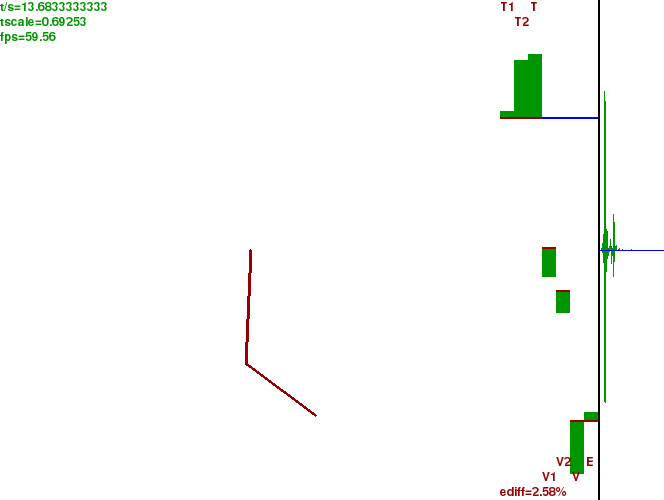
\includegraphics[width=0.7\textwidth]{images/haskell_simulation_fwindow1000_whitebg_cropped.png}
  \caption{Screenshot der Simulation}
  \label{fig:hssim}
\end{figure}

Zu erkennen ist die aktuelle Position des Pendels als rote Skizze der Arme.
Die dicken grünen Balken rechts daneben zeigen auf einer für alle dicken Balken gleichen Skalierung die Energien $T_1$, $T_2$, $T_{Ges}$, $V_1$, $V_2$, $V_{Ges}$ und $E_{Ges}$ in der Reihenfolge von links nach rechts an.
Der blaue Stricht zeigt die Nulllinie an, die roten Striche die Anfangswerte der Energien.
Die potentielle Energie ist anfangs kleiner als null, weil der Koordinatenurspung in der ersten Achse liegt und damit die Schwerpunkte der Pendelarme unterhalb des Bezugspunkts liegen.
Die Gesamtenergie $E_{Ges}$ sollte bei einer perfekten Simulation nicht von ihrem Anfangswert abweichen.
Werden die Schrittweiten für das Runge"=Kutta"=Verfahren kleiner als 10 Millisekunden gewählt, bleibt die Gesamtenergie in den ersten 60 Sekunden auch noch bis 8 Stellen nach dem Komma konstant.

Rechts neben den dicken Balken ist die diskrete Fourier"=Transformation der Winkel zu sehen.
Oberhalb der blauen Linie wird die Transformation von $\phi_1$ angezeigt, unterhalb die Transformation von $\phi_2$.
Jeder der Balken ist einen Pixel breit und bedeutet eine Frequenz aus dem Ergebnis.
Der Abstand nach rechts vom ersten Balken aus ist proportional zur Frequenz.
Aus dem aktuell zu sehenden Fester ist zum Beispiel für den ersten Pendelarm abzulesen, dass sich das Pendel regelmäßg von rechts nach links bewegt, zu erkennen am rechten Ausschlag, und der zweite Pendelarm eine schwächere aber schnellere Schwingung erzeugt, zu sehen als linker Ausschlag.

Die Transformation des zweiten Pendelarms zeigt eine starke Korrelation mit der Transformation des ersten Pendelarms. Das liegt daran, dass für diese Abbildung eine relativ stark periodische Einstellung des Systems gewählt wurde und der zweite Pendelarm eine dem ersten Pendelarm ähnliche Bewegung durchführt.

\begin{figure}
  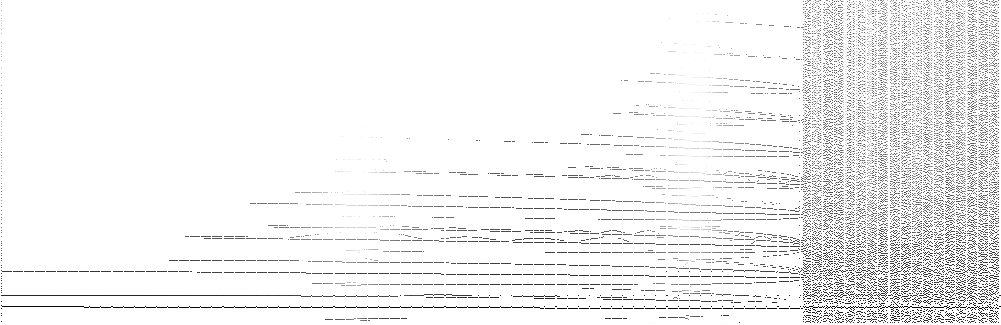
\includegraphics[width=\textwidth]{images/fourier_20s_cropped.png}
  \caption{Frequenzanalysen bei verschiedenen Startbedingungen. (Erklärung siehe Text)}
  \label{fig:frequencies}
\end{figure}

\subsection{Untersuchung des Frequenzspektrums}

\begin{wrapfigure}{r}{0.5\textwidth}
  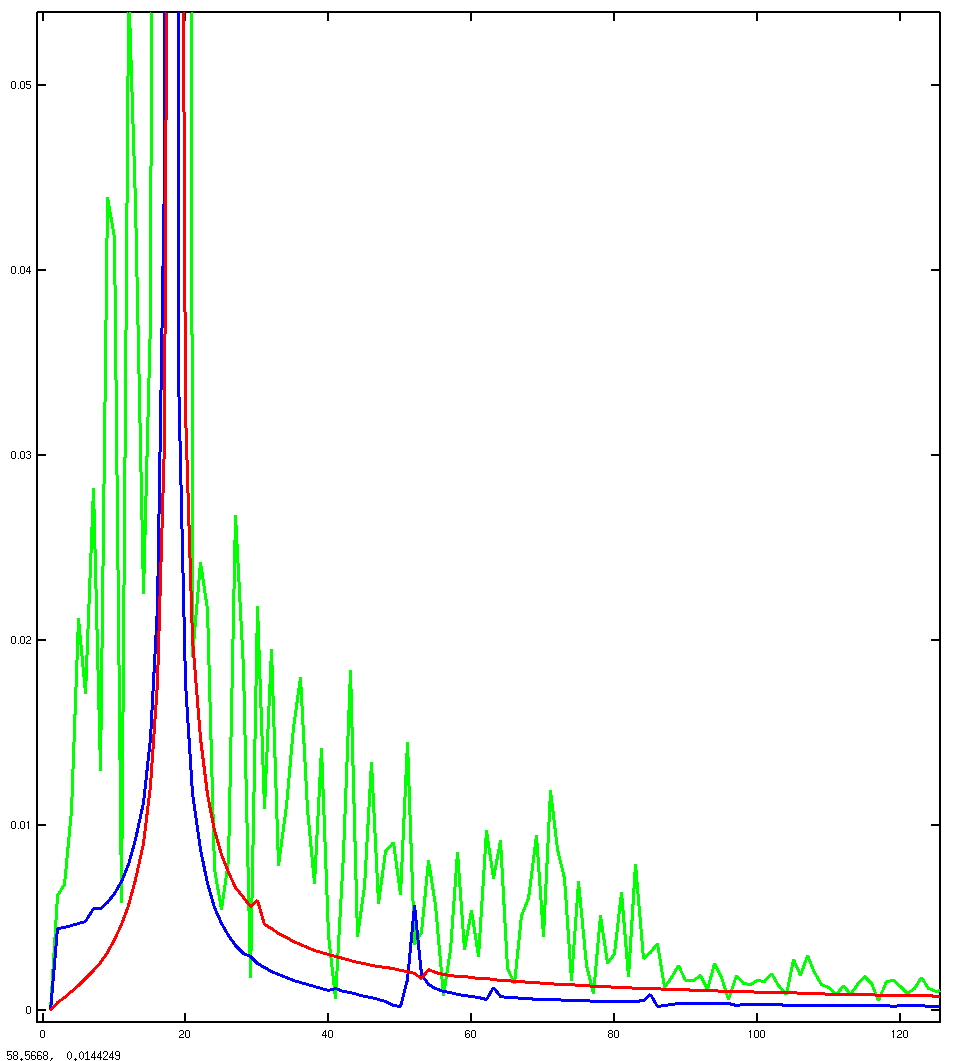
\includegraphics[width=0.5\textwidth]{images/fourier_100_400_900.png}
  \caption{Drei Fourieranalysen mit unterschiedlichen Startbedingungen.}
  \label{fig:fourieranalysen}
\end{wrapfigure}

Wenn die Simulation sehr oft durchgeführt wird und bei jeder Ausführung der Startwinkel $\phi_1$ um einen kleinen Schritt vergrößert wird, kann das Verhalten des Systems bei verschiedenen Energien untersucht werden.
Der Winkel des zweiten Pendelarms wird dabei immer mit der doppelten Größe initialisiert: $\phi_2 = 2\phi_1$.

In Abbildung \ref{fig:frequencies} ist ein Diagramm zu sehen, in dem von links nach rechts die Startbedingungen mit $\phi_1$ linear von $0\;rad$ bis $\pi/2\;rad$ vergrößert werden.
Auf der vertikalen Achse sind die Positionen der Maxima aus der Fourieranalyse für die ersten 20 Sekunden der Simulation aufgetragen.
Jeder Pixel der Grafik entspricht dabei einem Element aus der Fourierreihe.

Es sind mehrere Abschnitte zu erkennen, in denen unterschiedliche Muster vorherrschen.
Anfangs sind drei Maxima vorhanden, die den Frequenzen $0,5 Hz$, $1,5 Hz$ und $2,7 Hz$ entsprechen.
Hier sind die aus der Linearisierung berechneten Eigenfrequenzen wiederzufinden und eine Obschwingung, die zu beiden Frequenzen annähernd harmonisch ist.
Eine Fourier-Transformation aus diesem Bereich ist als rote Kurve in Abbildung \ref{fig:fourieranalysen} zu sehen.

Danach ist eine Verdopplung der Frequenzen zu beobachten, auf die immer mehr Oberschwingungen folgen.
Es sind zwischendurch auch Unterschwingungen zu beobachten.
Aus diesem Bereich stammt die blaue Transformation in Abbildung \ref{fig:fourieranalysen}.

Im rechten Teil des Diagramms ist zu erkennen, wie sehr kleine Änderungen in den Startbedingungen bei großen Energien so starke Abweichungen hervorrufen, dass sie sich sofort im Diagramm niederschlagen.
Dies ist der chaotische Bereich, aus dem die grüne Kurve in Abbildung \ref{fig:fourieranalysen} stammt.
Interessant ist, dass der chaotische Bereich immer wieder für bestimmte Anfangskonfigurationen sehr periodisch wird, wie an den senkrechten weißen Streifen zu sehen ist.

\begin{figure}
        \centering
        \begin{subfigure}[b]{0.32\textwidth}
                \centering
                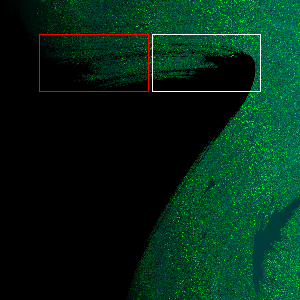
\includegraphics[width=\textwidth]{images/fraktale/loopgraph_300_300_marked.png}
                \caption{Gesamtes Diagramm}
                \label{fig:fraktale_gesamt}
        \end{subfigure}
        \begin{subfigure}[b]{0.32\textwidth}
                %phi1: 0.1990 - 0.7697
                %phi2: 2.1677 - 2.7855
                \centering
                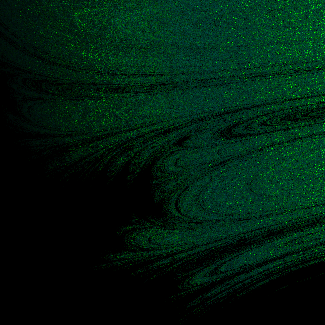
\includegraphics[width=\textwidth]{images/fraktale/ausschnitt_c.png}
                \caption{Roter Ausschnitt}
                \label{fig:fraktale_c}
        \end{subfigure}
        \begin{subfigure}[b]{0.32\textwidth}
                %phi1: 0.8011 - 1.3718
                %phi2: 2.1677 - 2.7855
                \centering
                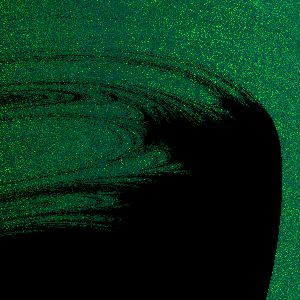
\includegraphics[width=\textwidth]{images/fraktale/ausschnitt_d.png}
                \caption{Weißer Ausschnitt}
                \label{fig:fraktale_d}
        \end{subfigure}
        \caption{Abbildungen der Übeschläge.}
        \label{fig:fraktale}
\end{figure}

\subsection{Abbildung der Überschläge}

Abhängig von den Startbedingungen kann auch die Anzahl der Überschläge des zweiten Pendelarms gezählt und in einem Diagramm farbkodiert aufgetragen werden.
An den Winkeln kann grob ein Überschlag abgelesen werden, wenn $\phi_2$ ein ungerades natürliches Vielfaches von $\pi$ überschreitet: $\phi_2 \in \{ \pm 1 \pi, \pm 3 \pi, \pm 5 \pi, ... \}$.
Denn genau dann zeigt das untere Pendel senkrecht nach oben und ein Überschlag ist sehr wahrscheinlich.

Da zum Erzeugen eines solchen Überschlagsdiagramms für jeden Pixel das Pendel über längere Zeit simuliert werden muss --- wir haben 60 Sekunden
als Simulationsdauer gewählt ---, ist es notwendig, die Simulationen sehr schnell ausführen zu können. Zu diesem Zweck haben wir zunächst mit der
C-Implementierung gearbeitet, die bereits weiter oben angesprochen wurde. Da aber auch diese auf einem Kern einer AMD-Brisbane-4400+-CPU
(Taktrate 2,3GHz) ca. 40 Minuten für die Simulation von 5000 Durchläufen benötigt, haben wir den C-Code für OpenCL umgeschrieben, sodass er
parallelisiert auf GPUs funktioniert. GPUs sind darauf optimiert, nach dem SIMD-Prinzip (Single Instruction, Multiple Data) zu arbeiten, das heißt, sie
können eine Operation parallel auf viele Datensätze anwenden\citep{gpuwiki}. Das passt zu unserem Problem, denn wir wollen die immer mit den gleichen
Operationen durchgeführte Simulation des Pendels mit vielen verschiedenen Startwerten laufen lassen. Mit dieser Methode erreichen wir auf einer
Radeon-HD-5750-Grafikkarte durch die SIMD-Ausführung des Codes Simulationsgeschwindigkeiten von ca. einer Minute für 5000 Durchläufe, was eine
Verbesserung um $97.5\%$ darstellt.

In Abbildung \ref{fig:fraktale} ist das Ergebnis von drei mal 90000 Durchführungen der Simulation mit 60 Sekunden Simulationszeit zu sehen.
Jedes Bild hat eine Auflösung von 300 mal 300 Pixeln, wobei auf der waagerechten Achse nach rechts $\phi_1$ und nach oben $\phi_2$ aufgetragen ist.
Der grüne Farbanteil codiert die Anzahl der Übeschläge nach links, der blaue Anteil die Überschläge nach rechts.
Weil die Startbedingungen nur auf einer Seite des Pendels (für Winkel größer Null) durchgeführt wurden, überwiegt die Anzahl der Überschläge nach links.

In Bild \ref{fig:fraktale_gesamt} ist $\phi_1$ im Intervall $[0; \pi/2]$ und nach oben ist $\phi_2$ im Intervall $[0; \pi]$ zu sehen.
Im schwarzen Bereich ist nicht genug Energie für einen Überschlag im System.
Interessant sind der blaue Bereich unten rechts, in dem überwiegend Überschläge nach rechts stattfinden, und der Bereich in der Mitte oben, in dem die Struktur zerfasert.
Zwei Ausschnitte aus diesem letzten Bereich sind in den Abbildungen \ref{fig:fraktale_c} und \ref{fig:fraktale_d} gezeigt.

In der Vergrößerung ist sehr schön ein fraktales Muster zu erkennen, das typisch für chaotische Systeme ist, wie zum Beispiel auch dem magnetischen Pendel. \citep{wikimagnetisch}

\subsection{Untersuchung des Phasenraums}

\begin{figure}
        \centering
        \begin{subfigure}[b]{0.3\textwidth}
                \centering
                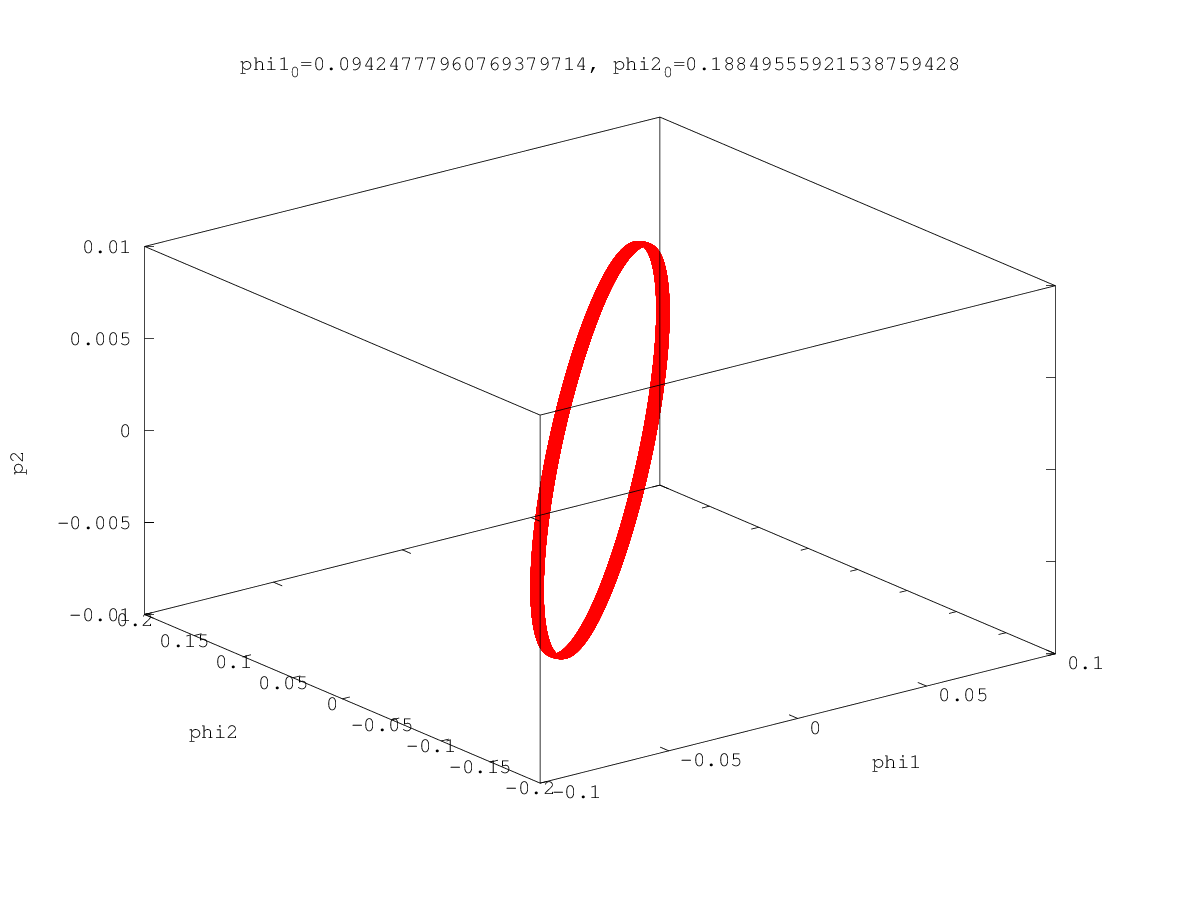
\includegraphics[width=\textwidth]{images/phasenraeume/phi2_is_2_phi1_6.png}
                \caption{Einfach periodischer Orbit}
        \end{subfigure}
        ~
        \begin{subfigure}[b]{0.3\textwidth}
                \centering
                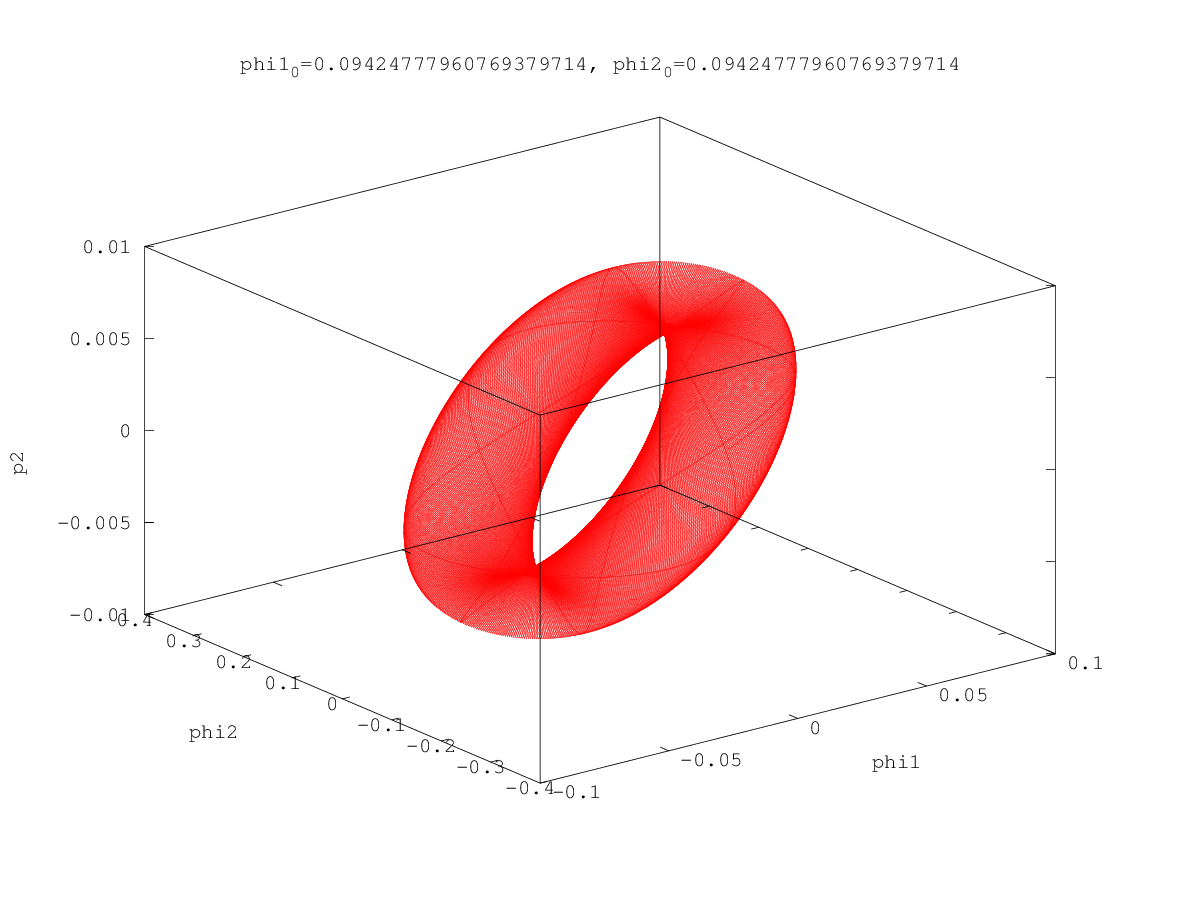
\includegraphics[width=\textwidth]{images/phasenraeume/phi1_is_phi2_6.png}
                \caption{Doppelt periodischer Orbit}
        \end{subfigure}
        ~
        \begin{subfigure}[b]{0.3\textwidth}
                \centering
                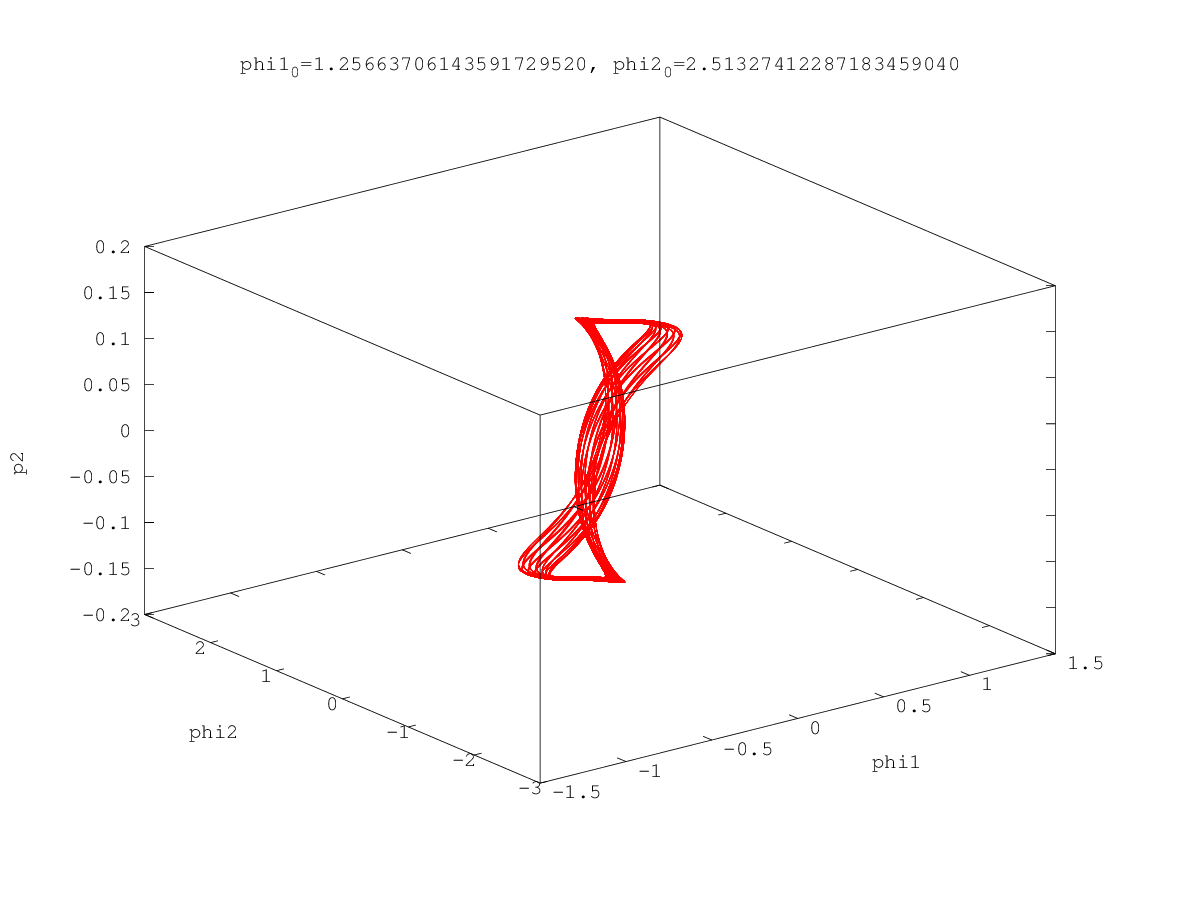
\includegraphics[width=\textwidth]{images/phasenraeume/phi2_is_2_phi1_80.png}
                \caption{Mehrfach periodischer Orbit}
        \end{subfigure}
        ~
        \begin{subfigure}[b]{0.3\textwidth}
                \centering
                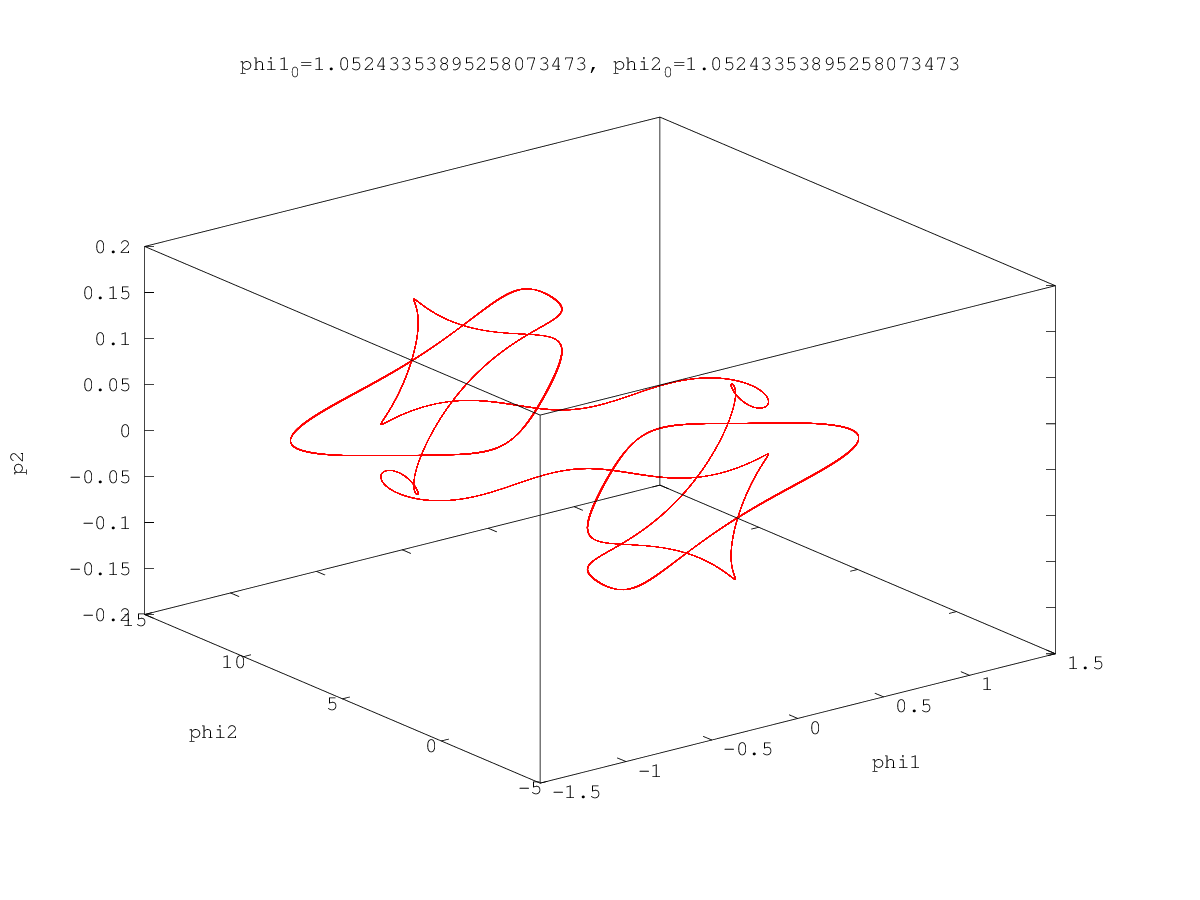
\includegraphics[width=\textwidth]{images/phasenraeume/phi1_is_phi2_67.png}
                \caption{Komplexerer Orbit}
        \end{subfigure}
        ~
        \begin{subfigure}[b]{0.3\textwidth}
                \centering
                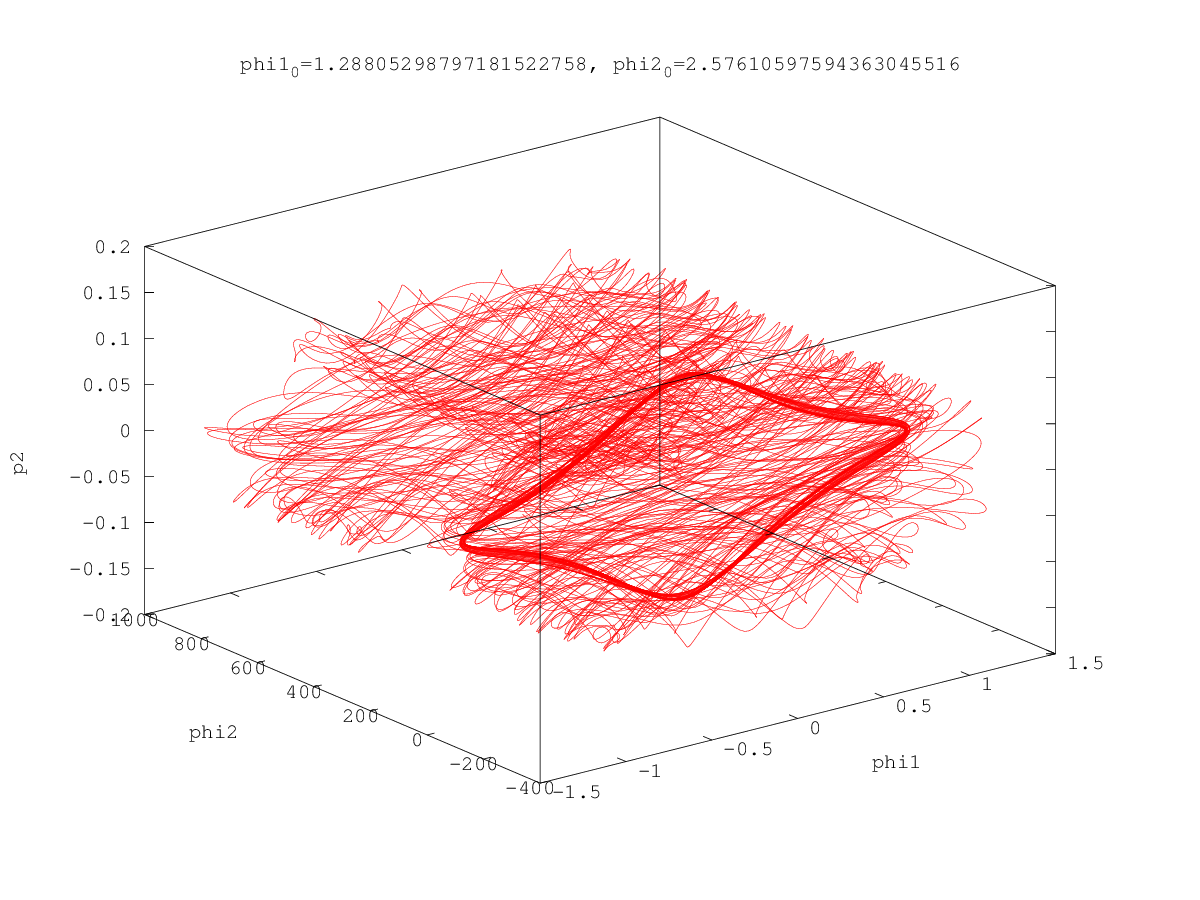
\includegraphics[width=\textwidth]{images/phasenraeume/phi2_is_2_phi1_82.png}
                \caption{Möglicher Attraktor}
        \end{subfigure}
        ~
        \begin{subfigure}[b]{0.3\textwidth}
                \centering
                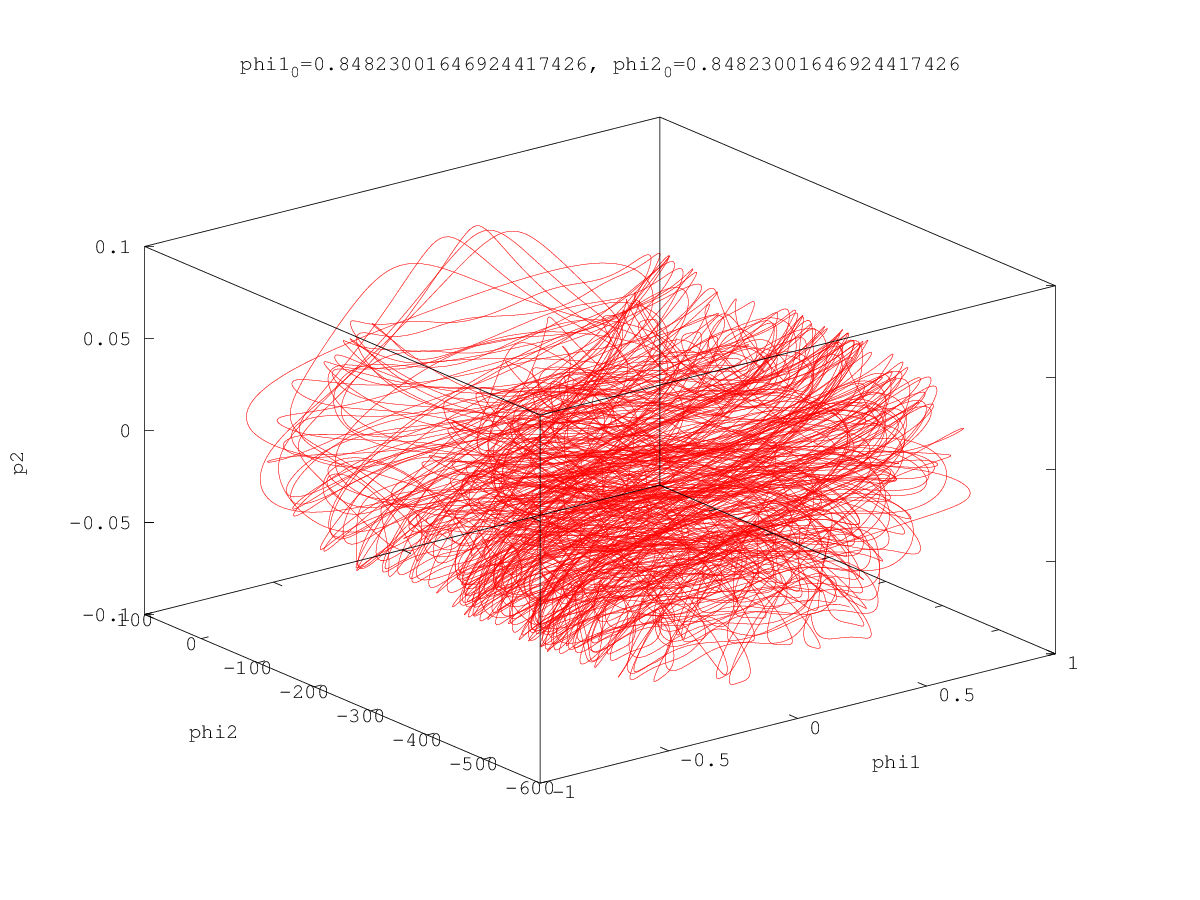
\includegraphics[width=\textwidth]{images/phasenraeume/phi1_is_phi2_54.png}
                \caption{Chaotischer Bereich}
        \end{subfigure}
        \caption{Trajektorien im kartesischen Koordinatensystem.}
        \label{fig:trajektorien_kartesisch}
\end{figure}

Die Bewegung des Pendels kann in einem dreidimensionalen Raum dargestellt werden.
Dabei wird auf jeder Achse einer der drei wichtigen Freiheitsgrade $\phi_1$, $\phi_2$ und $p_2$ aufgetragen.
Am einfachsten ist dabei die normale kartesische Darstellung.
In Abbildung \ref{fig:trajektorien_kartesisch} sind verschiedene interessante Orbits gezeigt.

Um aber die Periodizität der Winkel abbilden zu können, können Trajektorien auch in einem Torus gezeichnet werden, sodass $\phi_2$ auf der torodialen Achse, $\phi_1$ auf der poloidalen Achse und $p_2$ als Entfernung vom Mittelkreis des Torus dargestellt werden.
In Abbildung \ref{fig:vergleich_systeme} ist der Vergleich zwischen den beiden Darstellungsweisen gezeigt.
Die blauen Punkte geben die Begrenzung des Torus an.
Es ergeben sich Probleme wie dass zum Beispiel eine Achsenbeschriftung im Torus eher unübersichtlich ist und die Darstellung sehr gestaucht wird.
So ist auch der stark ausgeprägte periodische Bereich aus Abb. \ref{fig:vergleich_kartesisch} in Abb. \ref{fig:vergleich_torus} fast gar nicht mehr zu erkennen.

\begin{figure}
        \centering
        \begin{subfigure}[b]{0.49\textwidth}
                \centering
                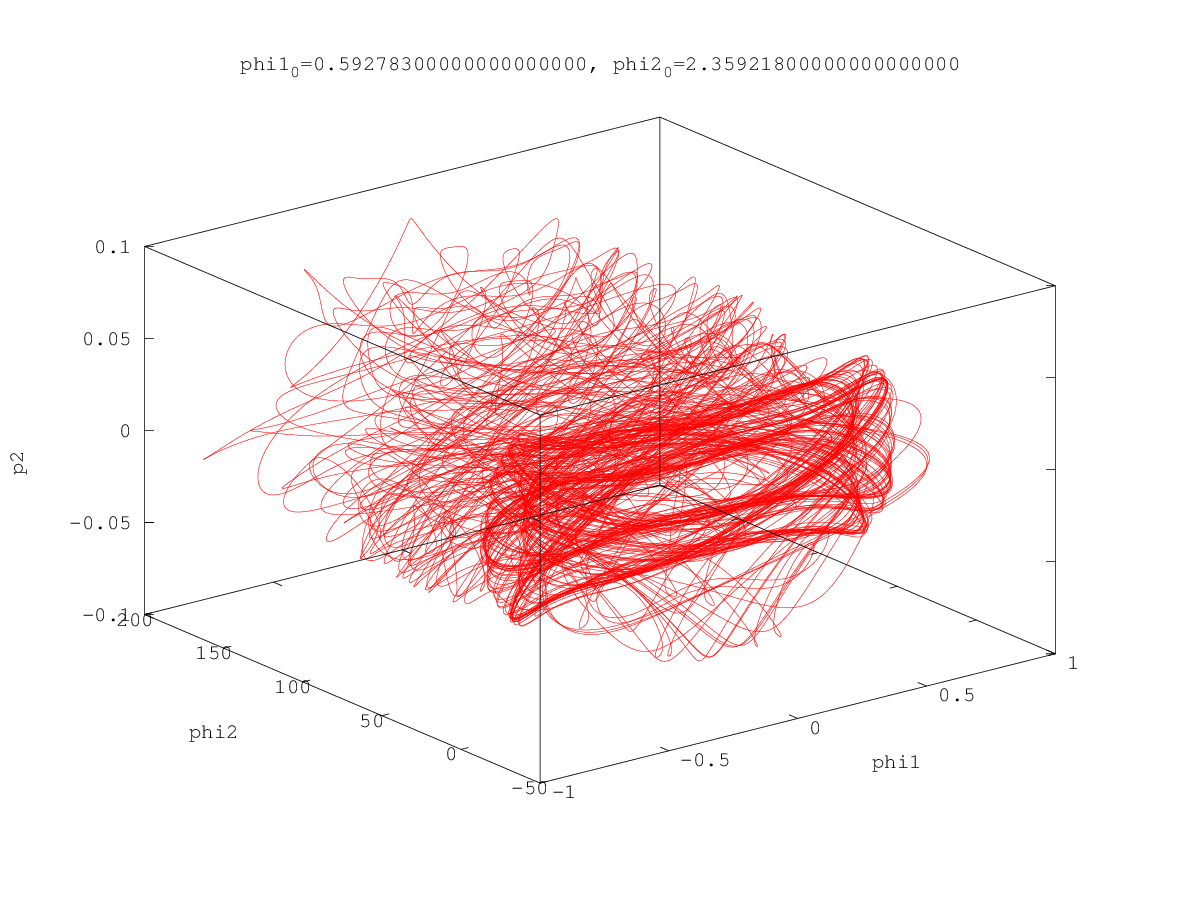
\includegraphics[width=\textwidth]{images/phasenraeume/c_diagonal_31.png}
                \caption{Darstellung im kartesischen Koordinatensystem}
                \label{fig:vergleich_kartesisch}
        \end{subfigure}
        ~
        \begin{subfigure}[b]{0.49\textwidth}
                \centering
                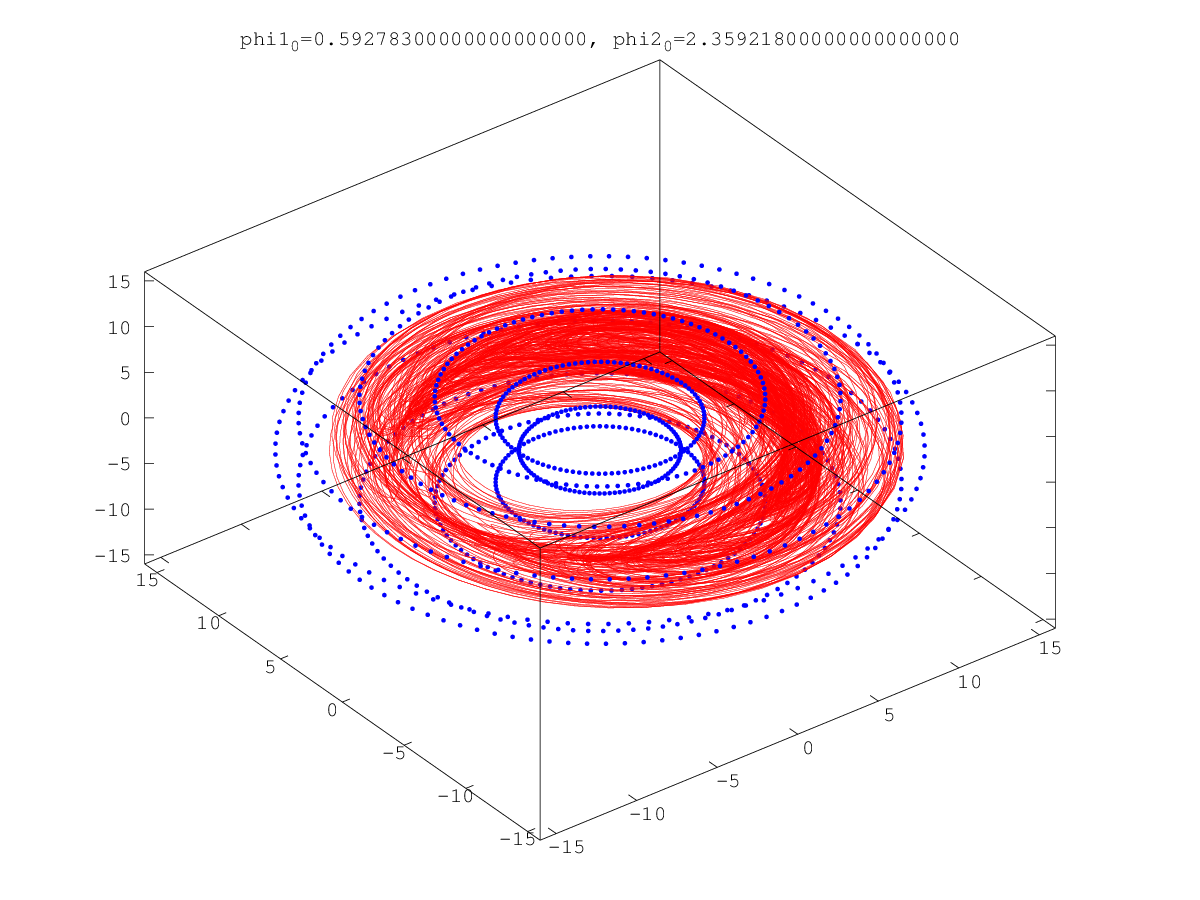
\includegraphics[width=\textwidth]{images/phasenraeume/c_diagonal_31_torus.png}
                \caption{Darstellung im Torus}
                \label{fig:vergleich_torus}
        \end{subfigure}
        \caption{Vergleich zweier gleicher Trajektorien.}
        \label{fig:vergleich_systeme}
\end{figure}



\section{Der Aufbau des Modells}

\begin{figure}
  \includegraphics[width=\textwidth]{charts/pendulumsketch.png}
  \caption{Position der Messspulen in Polarkoordinaten}
  \label{fig:pendulumsketch}
\end{figure}

Um das Verhalten des Doppelpendels zu beeinflussen, muss der Zustand des Pendels
erfasst werden können. Zu diesem Zweck verwenden wir einen am Ende des Pendels
befestigten Magneten, der in am Rahmen montierten Spulen elektrische Ströme
hervorruft, wenn er an diesen vorbeibewegt wird.

Diese Ströme verursachen Spannungsschwankungen an den Spulen. Um diese zu messen,
verbinden wir alle Spulen auf einer Seite mit einer 3,3 V--Span"-nungs"-quel"-le und auf der
anderen mit den 16 Analogeingängen eines ATmega2560--Mi"-kro"-con"-trollers. Der auf einen
Messbereich von 0 bis 5V eingestellte Mikrocontroller iteriert dann in einer Endlosschleife
über alle Eingänge, misst die an ihnen momentan anliegenden Spannungen mit einer
Auflösung von 10 Bit und leitet sie an einen Serial--to--USB--Konverter weiter. Der Messbereich
ist dadurch zwar relativ zur Grundspannung asymmetrisch --- der maximale negative Ausschlag beträgt
theoretisch 3,3 V, während der maximale positive Ausschlag $ 5V - 3,3 V = 1.7 V $ beträgt ---, aber
Spannungsregler für 3,3 V sind einfacher verfügbar als welche für 2,5 V.
% zusätzliches argument: negative spitzen machen mist?

Der Serial--to--USB--Konverter ist per USB an einen Computer angeschlossen, der die 5V--Stromversorgung
bereitstellt und die Messwerte aufzeichnen und verarbeiten kann.

Die 10--Bit--Auflösung des Mikrocontrollers bedeutet, dass die Schrittweite für die Digitalisierung
der Eingangswerte $ 5 V / 2^{10} = 4,883 mV $ beträgt. Da allerdings bei der Messung ein
Grundrauschen mit einer Breite von ca. XXXX V auftritt, ist die Genauigkeit der Messwerte geringer.

Aus Gründen der Einfachheit --- Atmel--Mikrocontroller mit USB--Schnitt"-stel"-le sind nur als SMD--Chips
verfügbar ---, haben wir uns dazu entschlossen, ein Arduino--Mega--2560--Board zu nutzen, das einen
ATmega2560--Mikrocontroller, einen ATmegaXXU2--Mikrocontroller als Serial--to--USB--Converter und eine 
3,3 V--Span"-nungs"-quel"-le enthält. Das Programm für den ATmega2560, das die Messwerte von den
Analogeingängen liest und über eine serielle Schnittstelle an den ATmegaXXU2 weitergibt, haben
wir aber selbst in C geschrieben, anstatt die Arduino--spezifische Sprache zu verwenden, die auf
einer höheren Ebene operiert, um möglichst gute Kontrolle über die Geschwindigkeit des Programms
zu haben.

Die Programmierung auf einer solch niedrigen Ebene und das Lesen der Mikrocontroller--Dokumentation
haben gezeigt, dass 500000 Baud die ideale Datenübertragungsrate für die Kommunikation mit dem PC
sind, da bei diesem Wert der Frequenzteiler für die serielle Datenübertragung genau 1 wird.
Tests mit dem in C geschriebenen Programm für den Mikrocontroller haben gezeigt, dass bei
dieser Baudrate die
parallel zur seriellen Datenübertragung ablaufende Analog--Digital--Wandlung die langsamste
Komponente ist, weshalb es ohne Leistungseinbußen möglich ist, für die Übertragung
der Messwerte an den PC ein Protokoll mit hoher Redundanz zu verwenden.

Das Protokoll zwischen Mikrocontroller und PC überträgt Messwerte als Kombination aus
Eingangs--ID und Messwert mit hoher Redundanz, sodass fehlerhafte oder
unerwartete Werte abgefangen und
ignoriert werden können. Solche fehlerhaften Werte sind zwar im laufenden Betrieb relativ selten,
treten aber während der Initialisierung des Arduino häufig auf. Ein weiterer Zweck der
mitgesendeten Eingangs--ID ist es, ohne bidirektionale Kommunikation eine Resynchronisation des
Empfängerprogramms auf dem PC beispielsweise nach einem Neustart zu ermöglichen.


\section{Messwertverarbeitung}
\begin{figure}
  \includegraphics[width=\textwidth]{charts/network_dia.png}
  \caption{Flussdiagramm der Messdaten}
  \label{fig:network}
\end{figure}

\clearpage
\addcontentsline{toc}{section}{Literatur}
\bibliographystyle{alphadin}
\bibliography{Dokumentation}{}

\end{document}

